\documentclass{article}

\usepackage{geometry, listings, amsmath,amsthm,amssymb}
\usepackage{graphicx}
\graphicspath{ {./pictures/} }

\geometry{
  tmargin = 20pt,
  bmargin = 35pt,
  textwidth = 590pt
}

\begin{document}

\begin{titlepage}
	\begin{center}
		\vspace*{2cm}
		
		\Huge
		\textbf{Post Office Simulation}
		
		\vspace{0.7cm}
		
		\vfill
		
		University of Exeter\\
		08/02/2021\\
		
	\end{center}
\end{titlepage}

\newpage

\section{Design decisions and assumptions}
\subsection{Global variable}
The variable shared\_r is the only global variable in this project. This is done only because this variable is needed for all of the gsl functions. A new random environment could be created and re-seeded everywhere where the gsl library is used but this is highly unnecessary and creates unnecessary overhead as well as redundant code.

\subsection{parameters file and terminal arguments}
To read in the parameters, it was chosen that the float type would be used as there is no need for the precision of a double in this simple simulation. For example, a difference of 0.001 customers arriving each minute is not likely to make a big difference in the result of each simulation.
The allowed parameters apart from the default ones are average new customers per interval, average customer wait limit, customer wait limit standard deviation, average customer serve time and customer serve time standard deviation. These parameters were added to allow for maximum customizability and flexibility in the simulations. Each parameter was made so that it can be specified by either a single value or a range in the format minValue $\sim$ maxValue. This is so that a number of simulations with some random parameters can be simulated to gather data quickly for the statistical analysis section. To accommodate this, the parameters are stored as an array of pairs.  
An extra optional terminal argument was also added which allows for repetition of the simulation, storing results in the experiments folder. So for example the command \$ testParams.txt 10 testOut.txt 100 would simulate using the parameters in the testParams.txt file a 100 times, creating a different result file for each of those 100 repetitions in the folder "experiments". This argument is optional and exists solely to make data gathering easier.

\subsection{Queue}
The queue structure and its related functions are made to be as generic as possible, that is, not restricted to this specific post office simulation project. This is evident in defining a customer type for items in the queue and the printQueue function which requires a function that prints an item within the queue. This approach was taken not only so this code could be used in other projects but also in case a queue that stores other structures or datatypes than customers was required.
Each node in the queue has a pointer to the next node and the previous node in the queue, effectively making it a doubly linked list. This design was chosen to make removing a node from the middle of the queue easier which is required when a customer times out and leaves the queue.
The queue has a head and tail attribute each pointing to the start and end of the queue respectively. This is done so adding items to the queue and dequeue-ing can be done without traversing the whole queue, thus reducing overhead.
A length attribute was added to the queue structure mainly for debugging purposes and for efficiency as this attribute allows for finding the length of the queue without traversing the whole queue.
Two approaches for the makeQueue function was considered – initialising with a value or not. It was decided to not initialise it with a value as the first value in the queue may not be known when creating the queue.

\subsection{Time unit}
In this simulation, it was decided that one time unit would represent one minute as it is a good compromise between accuracy and simplicity. This means the resolution for all the time elements within the simulation such as the time it takes to serve customers is one minute i.e. the time it takes to serve a customer cannot be 1 minute and 30 seconds. This is appropriate as any number that is not 1 such as 1timestep=10secs requires a conversion from timestep to real-world time units, which makes the code and thinking about the code quite confusing. Additionally, any unit smaller than a minute such as 1timestep=1second provides too much resolution and requires large numbers to represent timeframes such a typical working hour of 8hrs. Likewise, larger units provide not enough resolution.

\subsection{Statistical elements}
The gaussian distribution was chosen to set the time it takes for the customer to leave the queue(waitTime) and the time it takes for the customer to be served(serveTime) as these attributes are highly likely to be normally distributed in the real world. However, the attributes are cut off at 1 to remove any negative numbers and with the assumption that all customers will wait at least 1 minute and take 1 minute to serve. This is an appropriate as customers cannot be served instantaneously in the realworld. These parameters are not made adjustable in the parameters file as it is less likely these values would want to be adjusted, and shorter parameter file is more user friendly. Also, these values is unlikely to change the result of an experiment as long as it is kept reasonably small.
The poisson distribution was used to denote the number of customers that arrives each timestep. This allows the slight bypass of the time resolution being 1 minute as multiple customers may arrive in 1 minute using the poisson distribution. The exponential distribution was also considered as it requires decimal numbers to denote customers arriving in a sparse manner using the poisson distribution (e.g. a customer every 10 minutes with the poisson distribution requires lambda=0.1) which may be confusing. However with the exponential distribution, it is less straight forward to express multiple customers arriving in a minute.
The wait limit and serve time for customers are both rounded off to integers as even if they had decimal precision, the numbers would be rounded at some point since the minimum time step in the system is 1.
The data types for variables that are used for logging and writing the final output was made unsigned long just in case the user wanted to run a lot of simulations in a row. However,to minimise overhead, the variables that are only used in the simulations themselves are kept as integers so there is a potential for overflow if the user requests a large number of time steps in one simulation.

\section{Example output}
Here is an example of an output:\\
arriveRate, tillNum, maxLength, averageWaitLimit, waitLimitSD, averageServeTime, serveTimeSD \\
2.000, 1, 5, 20.000, 2.000, 3.000, 1.500\\
Average fulfilled customers: 37.500000\\
Average unfulfilled customers: 119.600000\\
Average timed out customers: 1.600000\\
Average of "Average wait time for fulfilled customers": 12.259226\\
Average time taken to empty queue after closing: 16.400000\\
\\
The top line lists the parameters in order to make reading the output easier.

\section{Statistics and experiments}
\subsection{Optimum number of service points and length of queue}
The aim in this section is to come up with a way of finding the optimum number of service points given the maximum length of the queue and the rate at which customers arrive. This objective was chosen since the length of the queue in a post office is unlikely to be changed and in this way, a post office branch can find the optimum number of service points if they know the rate at which customers arrive without running a number of simulations.
It was decided that the definition of "optimum number of service points" would be the minimum number of service points at which most customers would be served\: 95\% to be exact. This assumes a post office branch would prioritize serving customers than cutting costs.
To find this optimum point, a number of experiments were performed. Any simulation was simulated with 480 time steps to simulate a 8 hour working day and each simulation was repeated at least 100 times to average out any noise in the resulting data.

\subsubsection{Experiment 1: Arrive Rate}
In this experiment, the effect of the different arrive rates to the number of unfulfilled customers and timed out customers was explored. To do this, all parameters other than the arrive rate of customers are kept constant. For the average number of unfulfilled customers, a linear behaviour is expected once the queue becomes saturated and the rate at which customers arrives becomes larger than the ability of the post office to serve customers. This is because once the queue is saturated, (the rate at which customers arrive) - (the rate at which the branch serves customers) = (the rate of unfulfilled customers). For the average number of timed out customers, a constant value is expected as the queue saturates, since the number of customers in the queue at a given time will stay constant.
\begin{figure}[h]
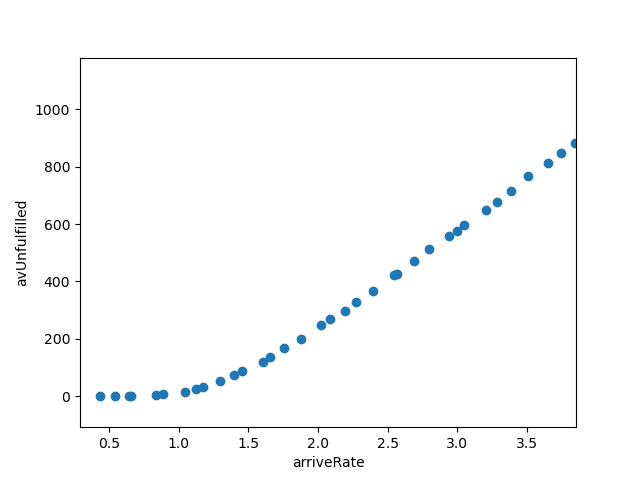
\includegraphics[width=5.8cm]{arriveRate_avUnfulfilled.png}
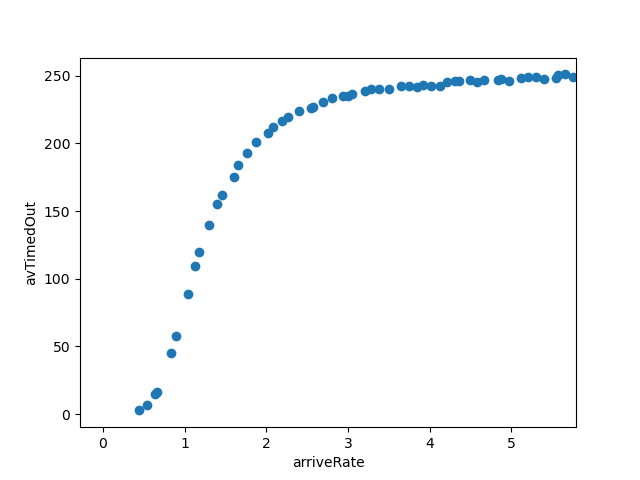
\includegraphics[width=5.8cm]{arriveRate_avTimedOut.png}
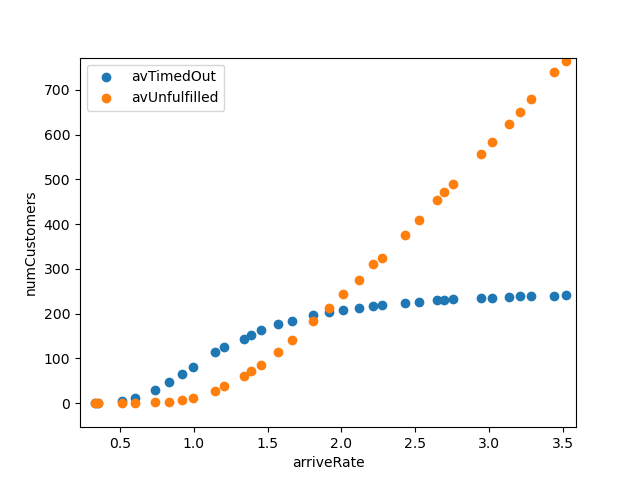
\includegraphics[width=5.8cm]{change_arriveRate.png}
\end{figure}
\\
The result is as expected where the number of unfulfilled customers seems to become directly correlated to the arrive rate at \(arriverate \approx 1.5\). So before this point, it seems minimizing the number of timed out customers is the most effective way to increase customer satisfaction, and after the crossing point, the number of unfulfilled customers should be the main concern.

\subsection{Experiment 2: Number of service points}
In this experiment, as well the arrive rate being changed, the number of service points are varied, and the same graphs as before are plotted. Increasing the number of service points means the rate at which the post office serves customers increase, thus reducing the queue growth rate. So we expect the point at which the two graphs linearise to shift to the right as the number of service points is increased.
\\
The graphs do behave as expected where as the number of service points are increased, the graphs linearise at a later point. However, there was a failure to predict that the number of timed out customers would plateau at a lower and lower number. From the graph, the plateau point is later than than when the graph of unfulfilled customers linearise, so it can be inferred that the average number of customers that time out plateaus after the queue is saturated. The saturation of the queue and the number of timed out customers being low could only mean the average wait time for customers is very low so most customers are satisfied, but the number of unfulfilled customers still increases so the queue must not be long enough to accommodate the arrive rate.
\begin{figure}[h]
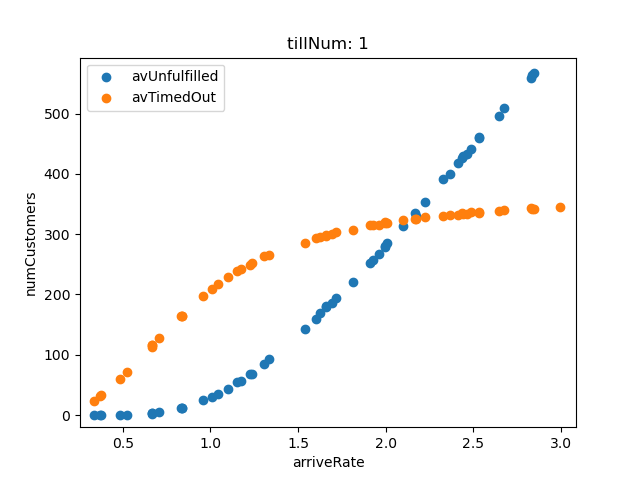
\includegraphics[width=5.9cm]{tillNum_1.png}
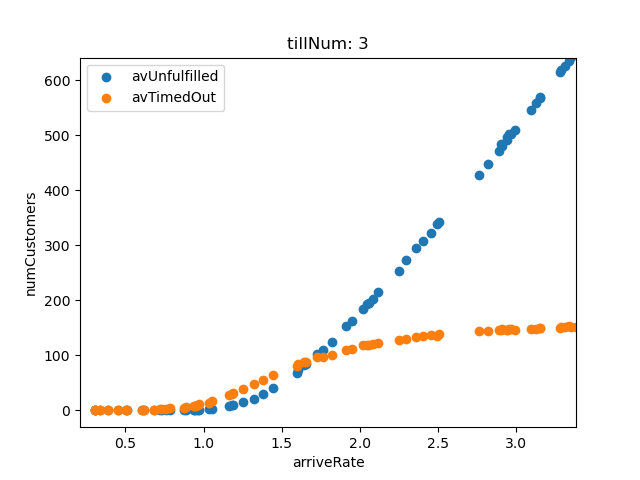
\includegraphics[width=5.9cm]{tillNum_3.png}
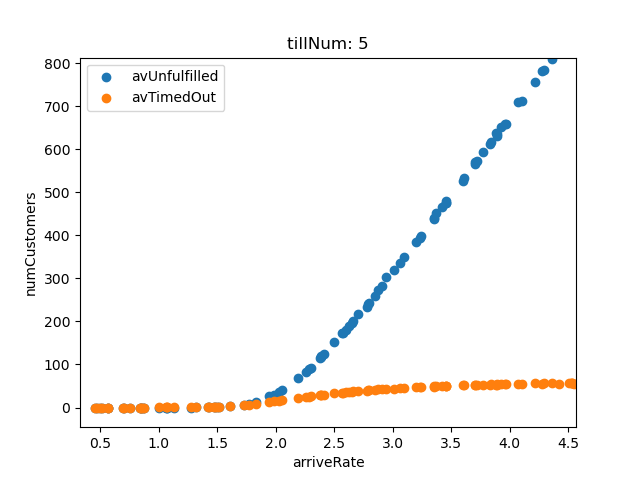
\includegraphics[width=5.9cm]{tillNum_5.png}
\end{figure}

\subsection{Experiment 3: Maximum length of queue}
This experiment is the same as experiment 2 but varying the length of the queue instead of the number of service points. A similar result for the number of unfulfilled customers as experiment 2 is expected. For the number of timed out customers, we expect to have a similar shape as in experiment 2 where it plateaus as the queue is saturated. However, we expect the value it plateaus at to increase the queue length is increased since more customers will join the queue and thus, customers have to wait longer on average.
\begin{figure}[h]
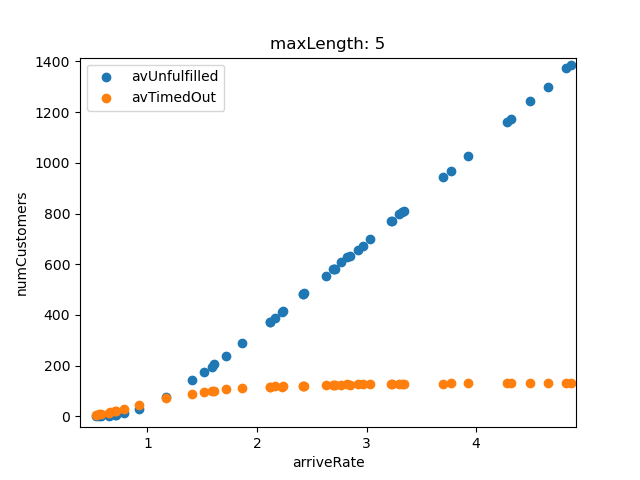
\includegraphics[width=5.9cm]{maxLen_5.png}
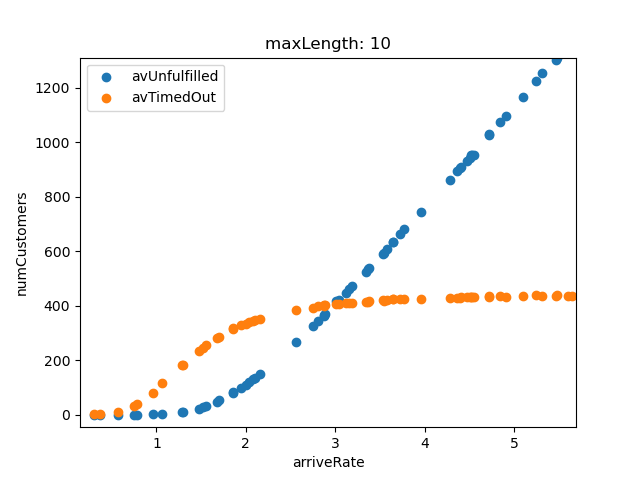
\includegraphics[width=5.9cm]{maxLen_10.png}
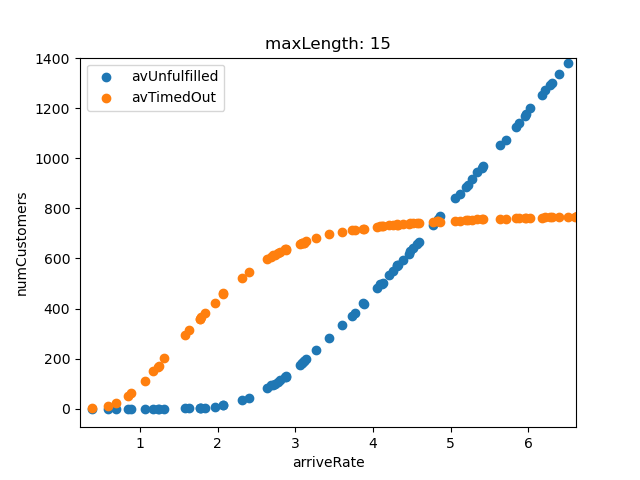
\includegraphics[width=5.9cm]{maxLen_15.png}
\end{figure}

\subsection{Experiment 4: Relation between length of queue and number of service points}
As how the length of the queue and number of service points impact the two variables we are trying to minimizing are understood, the best values in relation to the arrive rate of customers can be found. To find the relation between arrive rate and successful parameters, a number of simulations with different queue lengths, service points and arrive rates was performed to generate a heat map of queue lengths against service points at specific arrive rates with the heat value being the proportion of customers that are satisfied.
The following is a heat map of maximum queue length on the x-axis and number of service points on the y-axis for arrive rates of 4.6 and 6.2, where the red values indicate where the success criteria was met.
\begin{figure}[h]
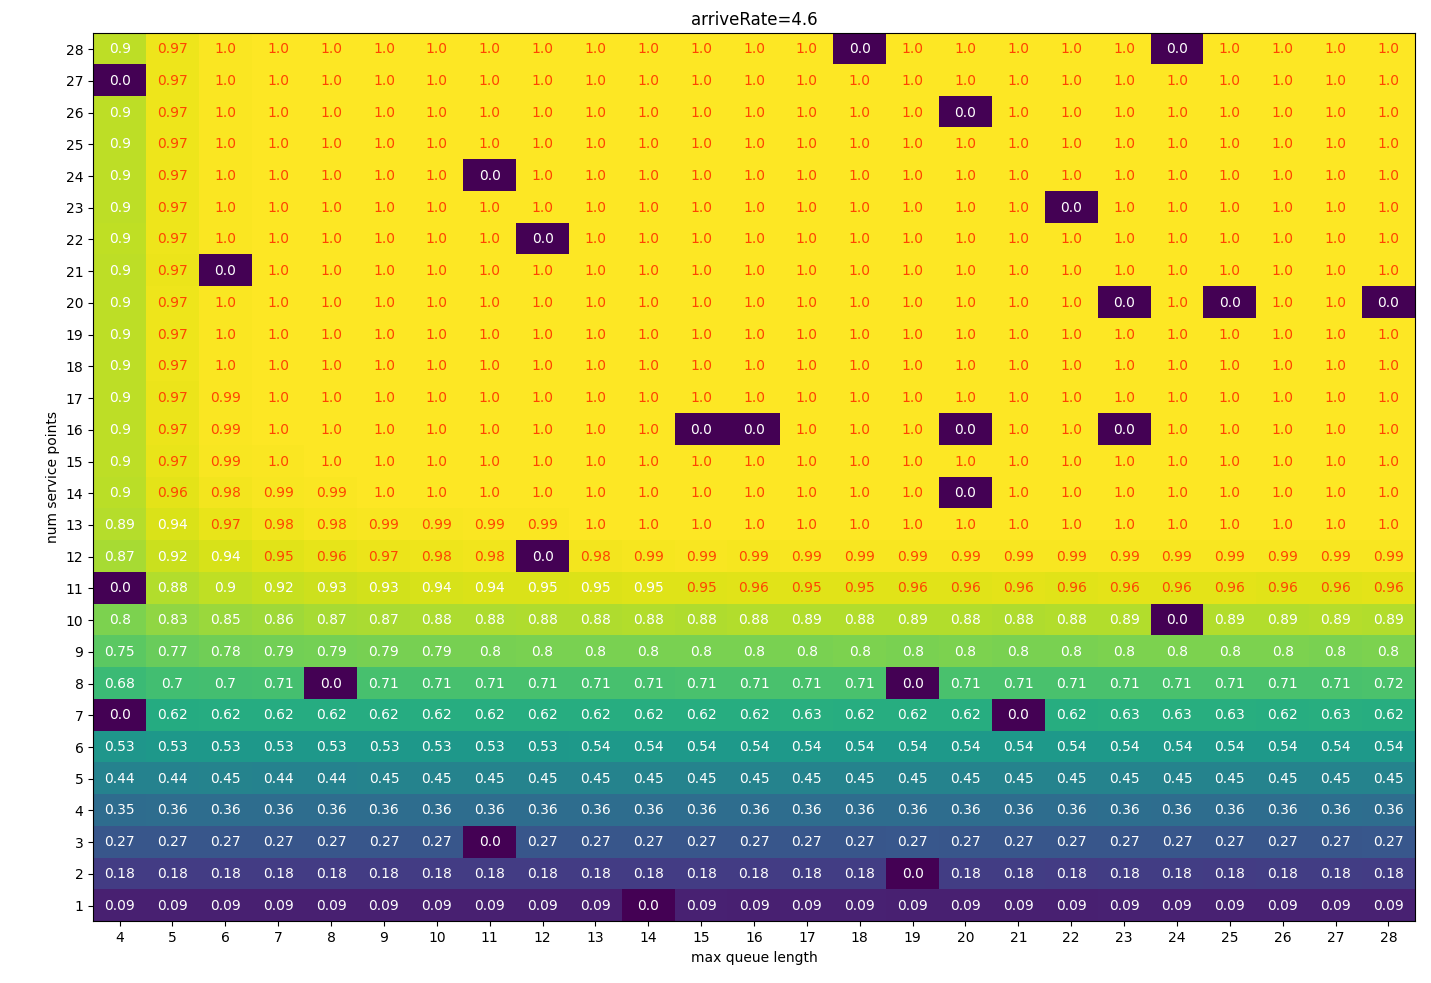
\includegraphics[width=9cm]{heat_map_4-6.png}
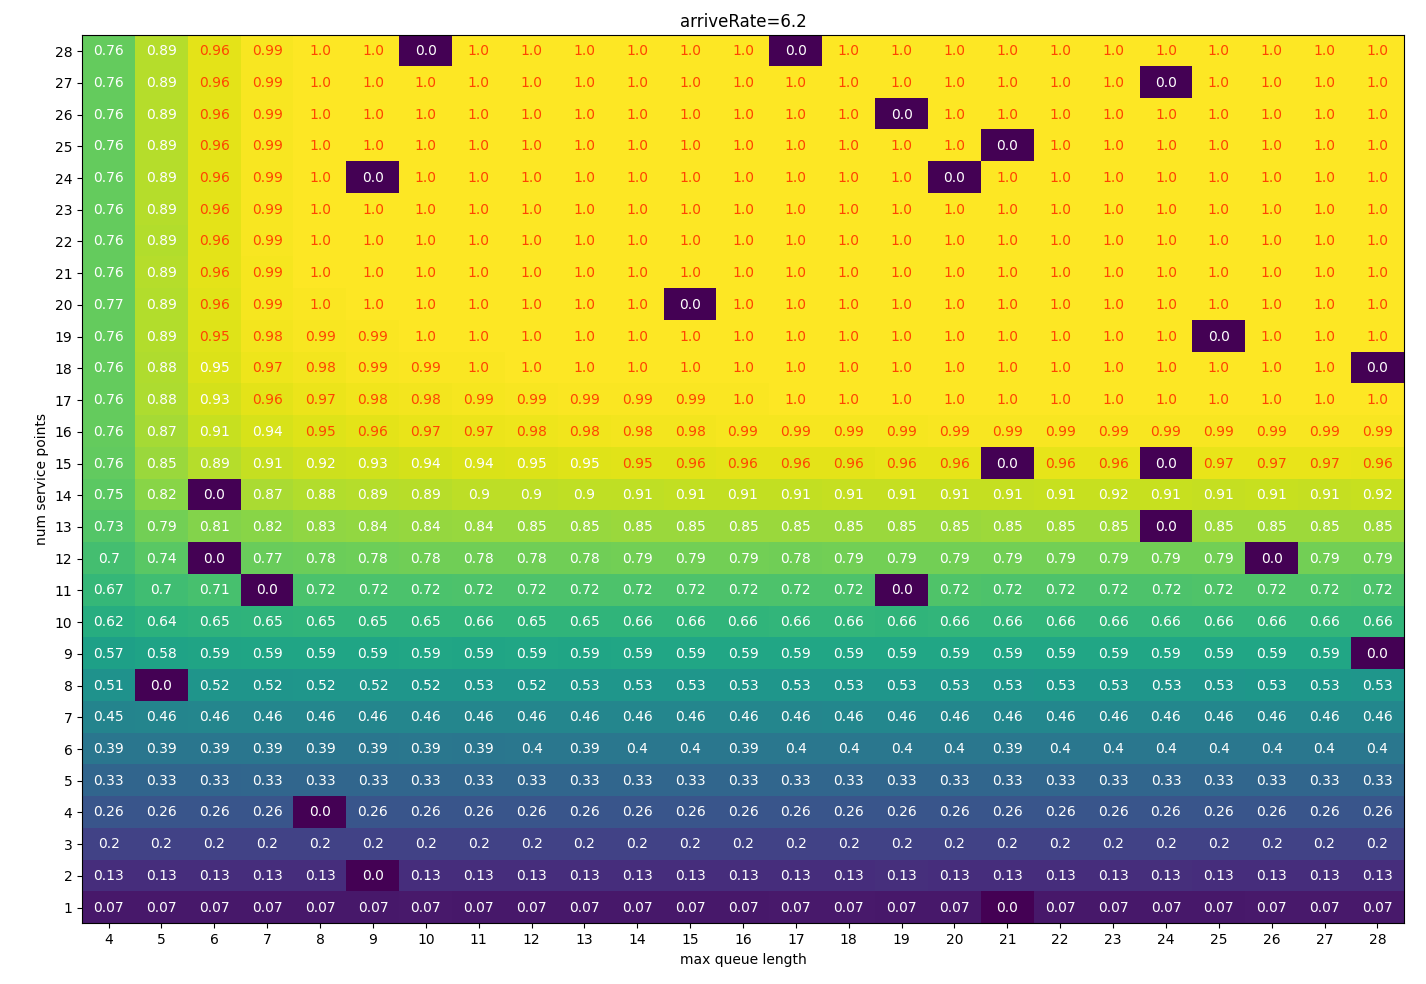
\includegraphics[width=9cm]{heat_map_6-2.png}
\end{figure}
\\
There are two key points to take away from the graphs. 1 - There is a minimum max queue length and minimum number of service points below which the simulation is not successful and above which, all simulations become successful. This means any extra number of service points or queue length is a waste and is not necessary. 2 - The boundary of successful simulations and non-successful ones seems to follow an equation of \(y=k/x + b\). The boundary of  successful and non-successful simulation identifies the minimum number of queue length needed for a certain number of service points and vice versa, therefore, by defining an equation for the boundary, a way of optimising number of service points from queue lengths can be found.


\subsection{Experiment 5: Equation for minimum queue length}
In the following experiments, the final formula is derived by first, finding the equation for the minimum queue length at which simulations first become successful, then finding the equation to model the boundary between successful and non-successful situations.
To find the minimum queue length and service points, the data gathered in the previous section was used to plot a graph of arrive rate against minimum values for arrive rate of 0.3 $\sim$ 10 in 0.1 increments. By plotting graphs of arrive rate against minimum queue length and arrive rate against minimum number of service points as well with their respective line of best fit, the following equation was derived.

For the queue length, let \(x=arrive rate, y=minimum queue length\) and it was observed that the conditional linear equation
\[
y = 
\begin{cases}
    4, & \text{if } x \leq 3.3,\\
    \text{round}(0.817x + 1.29), & \text{otherwise}
\end{cases}
\]
fits almost perfectly to the data points. This could mean the data points gathered are a small part of a larger, more complex equation but since the arrival rate of customers is unlikely to be much larger than 10 per minute, this approximation is appropriate.

\subsection{Experiment 6: Defining the boundary with an equation}
The aim of this experiment is to 1. Find a suitable equation for modelling the boundary shape between successful and unsuccessful parameters for the post office and 2. Find a general equation that comes up with the equation mentioned in 1. given an arrival rate of customers.

First the two coordinates of the corners (queueLength, numServicePoints) of the boundary were identified then, was used to calculate appropriate coefficients for the equation \(y=round(k/x+b)\). This equation was used to predict the boundary from queue lengths. Finally, the root mean squared error and mean absolute error was calculated to evaluate how appropriate the equation is for the given range. The graph of arrive rate against the error with this prediction method of the minimum number of service points showed that the root mean squared error(rmse) does not deviate far from the mean absolute error which indicates no big outliers and since the maximum absolute difference is around 0.9, and the maximum rmse was around 1.2. So the equation \(y=round(k/x+b)\) seems to be a good fit to model the boundary.
To derive this equation from the arrive rate, a graph of arrive rate against the variables k(left) and b(right) were plotted to see if there was a correlation.

\begin{figure}[h]
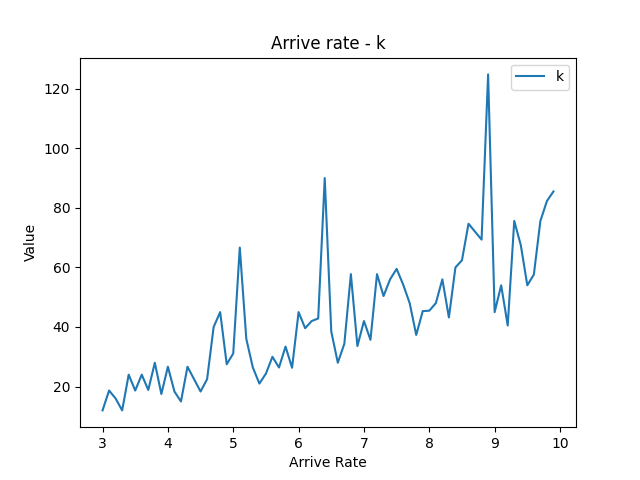
\includegraphics[width=8.5cm]{arrive_k.png}
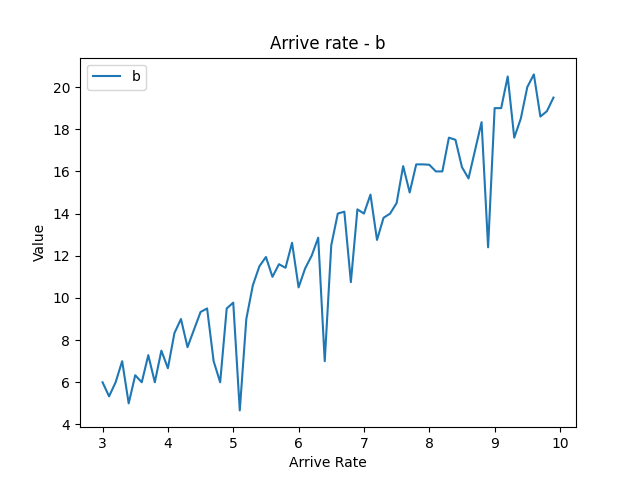
\includegraphics[width=8.5cm]{arrive_b.png}
\end{figure}

The graph unfortunately contains quite a bit of noise for the most suitable values for k and b. If a line of best fit is to be used for k and b it will increase the error but may still be a good method to predict the boundary. So a graph of arrive rate against error using the lines of best fit k = 10.22x - 15.64 and b = 2.137x - 0.93 was plotted and used to predict the boundary.
As expected, the errors increased, however the maximum rmse is less than 2.5 and surprisingly, the error seemed to plateau as the arriveRate increases so this model may still be suitable depending on the post office's tolerances. 
With this method, the final formula for the optimal number of service points is defined as follows:
Let y=number of service points, x=arrive rate, z=maximum queue length and m=minimum queue length.

\[
m = 
\begin{cases}
    4, & \text{if } x \leq 3.3,\\
    \text{round}(0.817x + 1.29), & \text{otherwise}
\end{cases}
\]

\[
k = 10.22x - 15.64,\\
b = 2.137x - 0.93\\
\]
\[
\begin{split}
\therefore
y = 
\begin{cases}
    inf, & \text{if } z < m,\\
    \text{round}(k/z + b) & \text{otherwise}
\end{cases}
\end{split}
\]
\end{document}